\documentclass[11pt]{article}
\usepackage{graphicx}
\usepackage[bookmarks=true]{hyperref}
\usepackage{bookmark}
\usepackage{hyperref}
\usepackage{csquotes}
\usepackage{float}
\usepackage{wrapfig}
\usepackage[normalem]{ulem}
\useunder{\uline}{\ul}{}

\usepackage{array}
\newcolumntype{L}[1]{>{\raggedright\let\newline\\\arraybackslash\hspace{0pt}}m{#1}}
\newcolumntype{C}[1]{>{\centering\let\newline\\\arraybackslash\hspace{0pt}}m{#1}}
\newcolumntype{R}[1]{>{\raggedleft\let\newline\\\arraybackslash\hspace{0pt}}m{#1}}

\setlength{\parindent}{0pt}

\begin{document}

\begin{titlepage}
\begin{flushright}


\includegraphics[width=380px]{../global/University_of_Pretoria_Logo.png}
\newline
\newline

\textbf {\LARGE Plan for Software Aspects of Certification} \newline

\textbf {\Large (PSAC)} \newline

\centering
\includegraphics[width=100px]{../global/Logo.jpg}

\textbf {\Large Linphone for Android Group Chat (Waterfall)}\newline

\flushright \textbf {\large Version: 1.2}\newline

\centering \textbf {\large Authors:}

\begin{table}[H]
\large
\centering
\begin{tabular}{rl}
	Izak Blom & 13126777 \\
	David Breetzke & 12056503 \\
	Paul Engelke & 13093500 \\
	Prenolan Govender & 13102380 \\
	Jessica Lessev & 13049136 \\
\end{tabular}
\end{table}

Date: \today

\end{flushright}
\end{titlepage}

\setcounter{tocdepth}{3}
\setcounter{secnumdepth}{5}
\tableofcontents

\newpage
\section{Revision History}
\begin{table}[h]
\begin{tabular}{llll}
\textbf{Date}          & \textbf{Description}  & \textbf{Author}       & \textbf{Comments}   \\ \hline
\multicolumn{1}{|R{2cm}|}{23/06/2015} & \multicolumn{1}{L{4.5cm}|}{Document Creation} & \multicolumn{1}{l|}{Team Eclectic} & \multicolumn{1}{L{4cm}|}{Version 1} \\ \hline
\multicolumn{1}{|l|}{} & \multicolumn{1}{l|}{} & \multicolumn{1}{l|}{} & \multicolumn{1}{l|}{} \\ \hline
\multicolumn{1}{|l|}{} & \multicolumn{1}{l|}{} & \multicolumn{1}{l|}{} & \multicolumn{1}{l|}{} \\ \hline
\multicolumn{1}{|l|}{} & \multicolumn{1}{l|}{} & \multicolumn{1}{l|}{} & \multicolumn{1}{l|}{} \\ \hline
\multicolumn{1}{|l|}{} & \multicolumn{1}{l|}{} & \multicolumn{1}{l|}{} & \multicolumn{1}{l|}{} \\ \hline
\multicolumn{1}{|l|}{} & \multicolumn{1}{l|}{} & \multicolumn{1}{l|}{} & \multicolumn{1}{l|}{} \\ \hline
\multicolumn{1}{|l|}{} & \multicolumn{1}{l|}{} & \multicolumn{1}{l|}{} & \multicolumn{1}{l|}{} \\ \hline
\multicolumn{1}{|l|}{} & \multicolumn{1}{l|}{} & \multicolumn{1}{l|}{} & \multicolumn{1}{l|}{} \\ \hline
\multicolumn{1}{|l|}{} & \multicolumn{1}{l|}{} & \multicolumn{1}{l|}{} & \multicolumn{1}{l|}{} \\ \hline
\multicolumn{1}{|l|}{} & \multicolumn{1}{l|}{} & \multicolumn{1}{l|}{} & \multicolumn{1}{l|}{} \\ \hline
\multicolumn{1}{|l|}{} & \multicolumn{1}{l|}{} & \multicolumn{1}{l|}{} & \multicolumn{1}{l|}{} \\ \hline
\multicolumn{1}{|l|}{} & \multicolumn{1}{l|}{} & \multicolumn{1}{l|}{} & \multicolumn{1}{l|}{} \\ \hline
\multicolumn{1}{|l|}{} & \multicolumn{1}{l|}{} & \multicolumn{1}{l|}{} & \multicolumn{1}{l|}{} \\ \hline
\multicolumn{1}{|l|}{} & \multicolumn{1}{l|}{} & \multicolumn{1}{l|}{} & \multicolumn{1}{l|}{} \\ \hline
\multicolumn{1}{|l|}{} & \multicolumn{1}{l|}{} & \multicolumn{1}{l|}{} & \multicolumn{1}{l|}{} \\ \hline
\end{tabular}
\end{table}

\section{Document Approval}
\begin{table}[h]
\begin{tabular}{llll}
\textbf{Signature}     & \textbf{Printed Name} & \textbf{Title}        & \textbf{Comments}     \\ \hline
\multicolumn{1}{|l|}{} & \multicolumn{1}{L{3.5cm}|}{} & \multicolumn{1}{L{3.5cm}|}{} & \multicolumn{1}{L{4cm}|}{} \\ \hline
\multicolumn{1}{|l|}{} & \multicolumn{1}{l|}{} & \multicolumn{1}{l|}{} & \multicolumn{1}{l|}{} \\ \hline
\multicolumn{1}{|l|}{} & \multicolumn{1}{l|}{} & \multicolumn{1}{l|}{} & \multicolumn{1}{l|}{} \\ \hline
\multicolumn{1}{|l|}{} & \multicolumn{1}{l|}{} & \multicolumn{1}{l|}{} & \multicolumn{1}{l|}{} \\ \hline
\end{tabular}
\end{table}

\newpage
\section{Stakeholders \& Developers}

Below is to be signed, acknowledgement of the contents of this document to be of acceptable standard and correct in terms of the requirements of the client.

\begin{table}[h]
\centering
\begin{tabular}{lll}
                              & \multicolumn{1}{L{3cm}}{} &    \multicolumn{1}{L{3cm}}{}    \\ \cline{1-1} \cline{3-3} 
Izak Blom (Developer)         &  & Date   \\
 & & \\
                              &  &        \\ \cline{1-1} \cline{3-3} 
David Breetzke (Developer)    &  & Date   \\
 & & \\
                              &  &        \\ \cline{1-1} \cline{3-3} 
Paul Engelke (Developer)      &  & Date   \\
 & & \\
                              &  &        \\ \cline{1-1} \cline{3-3} 
Prenolan Govender (Developer) &  & Date   \\
 & & \\
                              &  &        \\ \cline{1-1} \cline{3-3} 
Jessica Lessev (Developer)    &  & Date   \\
 & & \\
{\ul }                        &  & {\ul } \\ \cline{1-1} \cline{3-3} 
Kobus Coetzee (Client)        &  & Date  
\end{tabular}
\end{table}

\newpage
\section{Introduction}
\subsection{Purpose}
The purpose of this project is to extend Linphone's Instant Messaging (IM) implementation on Android platforms to include group chat and to implement other minor improvements to Linphones IM capabilities and user interface. \newline
This project also forms part of a larger Masters study on development methodologies for projects seeking DO-178 certification.
\newline \newline
The project will provide exposure to the following:
\begin{itemize}
\item Android development (Jave \& C),
\item open source contribution,
\item cryptography,
\item session initiation protocol (SIP),
\item and DO-178 certification.
\end{itemize}

\subsection{Scope}
The scope of this project will cover the following features to be added to the Linphone application for Android:
\begin{itemize}
\item providing group chat capabilities such as:
\subitem  - creation and deletion of groups,
\subitem  - adding and removing members,
\subitem  - broadcasting all messages to all members,
\item sending messages using AES256 encryption for secure messaging,
\item sending messages without encryption where it is not needed,
\item sending voice recordings over IM,
\item making changes to the messaging user interface such as:
\subitem  - improving the spacing between words,
\subitem  - increasing the font sizes,
\subitem  - improving message indentation for sender clarity,
\subitem  - adding indication of another user typing a message,
\subitem  - improving user profile picture displays.
\end{itemize}

\subsection{Documentation Conventions}
DO-178B does not specify the documentation standard to be followed, but most projects do follow some or other documentation standard. Figure \ref{figure-doc-con} is loosely based on \href{https://en.wikipedia.org/wiki/MIL-STD-498}{MIL-STD-490A}, although sometimes \textbf{Detail design} and \textbf{Notes} are changed into some other topic of discussion.
\begin{figure}[H]
\centering
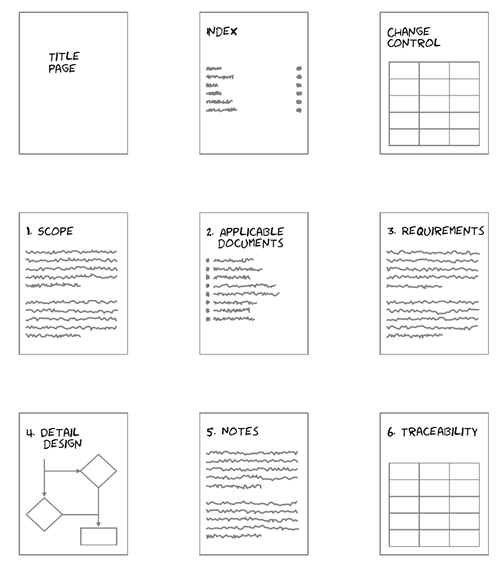
\includegraphics[scale=0.8]{./images/doc_convention.png}
\caption[Documentation Convention MIL-STD-490A]{A figure showing a documentation convention loosely based on MIL-STD-490A.}
\label{figure-doc-con}
\end{figure}

In the documentation, especially when talking about requirements and specifications, certain words convey additional meaning apart from their linguistic use. These words are usually capitalized.
\begin{itemize}
\item \textbf{\small \textit{SHALL}} and \textbf{\small \textit{SHALL NOT}} - Indicates a mandatory requirement.
\item \textbf{\small \textit{WILL}} and \textbf{\small \textit{WILL NOT}} - Indicates a declaration of purpose or an expression of simple futurity.
\item \textbf{\small \textit{SHOULD}} and \textbf{\small \textit{SHOULD NOT}}- Indicates a non-mandatory desire, preference or recommendation.
\item \textbf{\small \textit{MAY}} and \textbf{\small \textit{MAY NOT}} - Indicates a non-mandatory suggestion or permission.
\item \textbf{\small \textit{MUST}} and \textbf{\small \textit{MUST NOT}} should be avoided as it causes confusion with the above terms. 
\end{itemize}

\section{System Overview}
\subsection{Server Architecture}
Linphone makes use of a Flexisip server. Flexisip is compliant with RFC3261 and written in C++11.\\

Flexisip makes use of a modular architecture with limited dependencies to allow it to run smoothly on small devices/hardware. Requests and responses are processed through a chain of modules, where each module is typically responsible for a single task such as registration, media relay, authentication, etcetera. \\

Flexisip provides the following main features according to \href{www.linphone.org}{the Linphone website}:
\begin{itemize}
\item transport protocols (SIP/UDP, SIP/TLS, SIP/TCP),
\item NAT awareness with a built-in media relay module and stun server,
\item digest authentication using an external SQL password or static password file,
\item a registrar, that among other things stores the address of record to allow routing to clients that register,
\item routing based on the registrar database or a static file, with forking,
\item interconnected with push notification systems that allows for reliable notifications of incoming calls and messages to mobile clients,
\item high level event logging for monitoring purposes,
\item and cluster mode operation for large deployments.
\end{itemize}

Flexisip's cluster mode involves using several proxies in combination for scalability and fault tolerance. This requires the use of a fault-tolerant Redis database, DNS-SRV records and multiple Flexisip instances (on separate  machines).

\section{Software Overview}
\subsection{Software Architecture}
Linphone utilises a layered approach to the architecture, allowing for a separation between the user interfaces and the core engine. This allows various interfaces to be created on a higher layer drawing on functionality from the lower layers.
\\
The highest layer consists of the different user interface front-ends (Android, iPhone, Windows, etc.) along with bindings or plugins related to the next layer.
\\
The next layer is Liblinphone which is a library which implements all functionality of used by the user interfaces. It forms the core engine and allows Linphone or any application to initial, receive, terminate audio and video calls due to Liblinphone being cross-platform.
\\
Liblinphone relies on following parallel layers to provide software components to the library. These layers consist of a multimedia SDK to process and stream audio/video (Mediastreamer2), a simple real-time transport protocol for delivering audio/video over IP networks, and a Session Initiation Protocol library for signalling and controlling multimedia communication sessions.

\subsection{Extension Architecture}
\subsubsection{Preface}
It is our intention to develop the Linphone Group Chat extension as a subsystem that is decoupled from the existing system to the greatest extent possible. Hence, our aim is to write a subsystem using an architecture that is effectively hides the extension from the rest of the architecture with minimal changes to existing code to incorporate the extension.

\subsubsection{Decentralisation}
To maintain Linphone's server independence, we have elected to develop the extension to behave as a distributed system such that no changes need to be made to server functionality to incorporate the additions to the client. While this may be more complex than centralising the group chat subsystem as a server level, we have had to factor in the constraints we have on time as changing a server would increase the scope of the project drastically as well as risk to project success.

\subsubsection{Related Architecture}
We are focused on developing a modular system, and a component-based architecture suits our needs. While some of the core functionality requires knowledge of the existing Linphone system, we aim to implement our low level components as completely decoupled from the extension core and thus the Linphone core. Figure \ref{figure-architecture} shows the general design for the subsystem.
\begin{figure}[H]
\centering
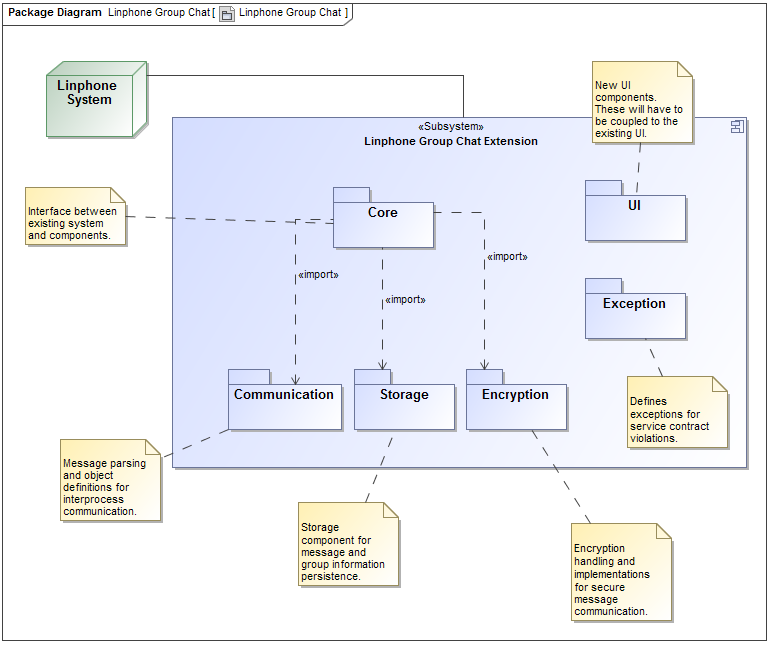
\includegraphics[width=5in]{./images/architecture.png}
\caption[Architecture UML]{A diagram showing the general design of the Linhpone Group Chat Extension.}
\label{figure-architecture}
\end{figure}

\subsubsection{Patterns}
\paragraph{Inversion of Control}
We will be making use of dependency inject to further decouple the components from some of the core functionality. 
\paragraph{Factory Pattern}
Construction of components will be delegated to factory classes in each of the component modules. The use of these factories will also facilitate mandatory conformance of component implementations to the interfaces they realise as well as hide concrete implementations from the client components.
\paragraph{Strategy Pattern}
Strategies will be used to provide different implementations of encryption algorithms to allow flexibility and accommodate user needs or preferences.

\section{Certification Considerations}
The project will be developed according to DO-178 certification requirements, for level D certification. Justification for level D is not dependent on safety considerations as is usually the case, but rather on limited time and the limited experience the team has with DO-178. \\ \\
This project is not intended for avionics applications and is not safety critical, but rather serves as a case study on DO-178 software development.

\section{Software Lifecycle}\label{sec:soft-life}
A waterfall software development methodology will be followed with this project. Figure \ref{figure-waterfall} shows a simple model of the development process that will be followed for this project.

\begin{figure}[H]
\centering
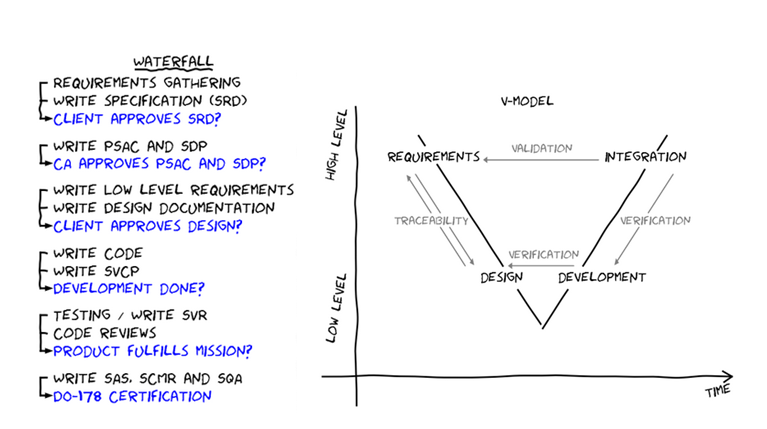
\includegraphics[width=4.5in]{./images/waterfall_model.png}
\caption[Waterfall Model]{A figure showing the development process for this project.}
\label{figure-waterfall}
\end{figure}

\subsection{Traceability}
The purpose of traceability is foremost to ensure that the design takes into account all the requirements set for the project. Requirements which have not been taken into account by the design are called \textbf{childless} requirements.\\

Traceability analysis must also ensure that there are no additional, unnecessary requirements introduced during the design phase as they may escalate the development costs. Such requirements are called \textbf{orphan} requirements. \\

For these reasons, most of the documentation for this project will contain a traceability matrix that will indicate the relationships between requirements.

\subsection{Verification}\label{subsec:verification}
Verification is concerned with whether or not the product is being implemented correctly according to the design, and whether or not integration is  being done correctly according to the design and the development process. \\

Verification for DO-178 consists of two steps, namely:
\begin{itemize}
\item Requirements-based Coverage Analysis, where it is checked if all requirements are satisfied and tested;
\item and Structural Coverage Analysis, where it is checked that, during testing, all paths are executed and that no code in the final product is untested.
\end{itemize}

Lastly, as part of the DO-178B verification process, it is required that there be no dead code present in the final binary and that de-activated code (perhaps code used in another configuration of the product) cannot be accidentally activated.

For these reasons, code coverage tests are required for the various levels of DO-178:
\begin{itemize}
\item Level A requires \href{https://en.wikipedia.org/wiki/Modified_condition/decision_coverage}{Modified Condition Decision Coverage (MCDC)}.
\item Level B requires decision coverage.
\item Level C requires coverage of dependencies.
\item Level D requires no code coverage verification.
\end{itemize}

\subsection{Validation}
Validation is concerned with whether or not the final product satisfies the intended use of the product, i.e \enquote{Did we build the right thing?} or \enquote{Does this product actually work?}. Sometimes this is not the case.

\section{Software Development Environment}
Development for this project will be done under the following conditions:\\
\begin{itemize}
\item \textbf{Operating System} \\
The Linux operating system will be used as a platform for development.\\
\item \textbf{IDE} \\
Eclipse will be used as an IDE.\\
\item \textbf{Programming Language} \\
Looking at the current state of Linphone:\\
The iPhone application is built in objective C.\\
The Android application is built to run using Java.\\
The Windows phone application is built using C\#.\\
\\
For this specific extenion of Linphone:\\
Since the extension is done for Android, Java will be used as the main programming language. Exposure to C will also take place.\\
\item \textbf{Other Tools} \\
For this specific extension tools such as Android Developer Tools (ADT) will be used.\\
\item \textbf{Testing} \\
Technology such as JUnit will be used for testing.\\
\end{itemize}
\section{Software Lifecycle Data}
The following deliverables will be created during this project:
\begin{itemize}
\item \textbf{Plan for Software Aspects of Certification (PSAC)} \\
The Plan for Software Aspects of Certification is the primary means used by the certification authority for determining whether an applicant is proposing a software life cycle that is commensurable with the rigour required for the level of software being developed.
\item \textbf{Software Development Plan (SDP)} \\
The Software Development Plan includes the objectives, standards and software life cycle(s) to be used in the software development processes.
\item \textbf{Software Verification Plan (SVP)}
The Software Verification Plan is a description of the verification procedures to satisfy the software verification process objectives.
\item \textbf{Software Requirements Data or Specification (SRD/SRS)} \\
Software Requirements Data is a definition of the high-level requirements including the derived requirements.
\item \textbf{Software Design Description (SDD)} \\
The Software Design Description is a definition of the software architecture and the low-level requirements that will satisfy the software high-level requirements.
\item \textbf{Source Code} \\
This data consists of code written in source language(s) and the compilation instructions for generating the object code from the source code, and linking and loading data. This data should include the software identification, including the name and date of revision and/or version, as applicable.
\item \textbf{Executable Object Code} \\
This data consists of code written in source language(s) and the compiler instructions for generating the object code from the Source Code, and linking and loading data. This data should include the software identification, including the name and date of revision and/or version, as applicable.
\item \textbf{Software Verification Cases and Procedures (SVCP)} \\
Software Verification Cases and Procedures detail how the software verification process activities are implemented.
\item \textbf{Software Verification Results (SVR)} \\
The Software Verification Results are produced by the software verification process activities.
\item \textbf{Software Accomplishment Summary (SAS)} \\
The Software Accomplishment Summary is the primary data item for showing compliance with the Plan for Software Aspects of Certification.
\end{itemize}

\section{Software Development Plan}
\subsection{Software Development Approach}
As stated in Section~\ref{sec:soft-life} The waterfall model shall be used in this project.
Development activities will be performed in order, with possibly minor overlap, but with little or no iteration between activities. User needs are determined, requirements are defined, and the full system is designed, built, and tested for ultimate delivery at one point in time. This is a document-driven approach.

\subsection{General Plans for Software Development}
Software development will follow a prioritised list. Team Eclectic will iteratively develop functionality in order of priority. Development is to be done both during group meetings, and also remotely by making use of the private git repository.
\subsubsection{Development Standards}
The Android Linphone application is written in Java. Each Java file is preceded by a license comment. Internal code documentation is currently minimal, and comments are used to highlight quick-fixes for known problems. We will adhere to the highly-descriptive function and class names which are used throughout Linphone. \\
Internal Java documentation will be focused upon. Class descriptions will be provided as well as descriptions for functions, along with their parameter lists, return values and exceptions.
\subsubsection{Patterns \& Frameworks}
Modularity is a major focus in the Linphone application. We will continue this approach. Waterfall typically follows long release-cycles and the development framework will not be iterative, as one development cycle will be performed. Emphasis will be on completing each job correctly "First-time around". \\ 
Also we will be making use of dependency injection as to promote testing and decrease coupling between classes and their dependencies.
\subsubsection{Testing}
Unit testing will be done on every new component. This is necessary to adhere to the DO-178 verification level D for code coverage as outlined in Subsection~\ref{subsec:verification}.\\
Once we have created the necessary classes and interfaces, unit tests will be established using JUnit. This will be done to ensure that any violations of the requirements and any errors are caught from the beginning and to ensure that code always meets the requirements.

\section{Licensing \& Ownership}
This project extends an open-source project by Belledonne Communications and is thus also itself intended to be open-source. To this end the permissions will be sought from the University of Pretoria.

\end{document}